\chapter{AspectJ Code Generation}
\label{chapter:codeGeneration}

\begin{flushright}
\textit{Chapter written by Claas Wilke}
\end{flushright}

This Chapter describes how the Java Code Generator \keyword{OCL22Java} provided with \acl{DOT4Eclipse} can be used. A general introduction into \acl{DOT4Eclipse}  can be found in Chapter \ref{chapter:introduction}. A detailed documentation of the development of OCL22Java can be found in the Minor Thesis (Gro�er Beleg) of Claas Wilke \cite{GB:Wilke}.

In addition to the general Eclipse installation the \keyword{\acf{AJDT}} are required to execute the code generated with OCL22Java. The \acs{AJDT} plug-ins can be found at the \acs{AJDT} website \cite{WWW:AJDT}. 
  


\section{Code Generator Preparation}

This Chapter uses the \keyword{Simple Example} which is provided with \acl{DOT4Eclipse} and has been introduced in Subsection \ref{intro:simpleExample} To import the Simple Example into our Eclipse workspace we have to create a new Java project into our Workspace (here called \model{tudresden.ocl20.pivot.\linebreak[0]examp\-les.\linebreak[0]simple}) and use the import wizard \eclipse{General -> Archive File} to import the example provided as a \acs{JAR} archive. In the following window we select the directory were the \acs{JAR} file is located (probably the \model{plugins} or \model{dropins} directory inside the Eclipse root folder). We select the archive \model{tudresden.ocl20.pivot.\linebreak[0]examples.simple.jar} and click the \eclipse{Finish} button (if you use a source code distribution of \acl{DOT4Eclipse} instead, you can simple import the project \model{tudresden.ocl20.pivot.examples.simple} using the import wizard \eclipse{General -> Existing Projects into Workspace}).

Next, we have to import a second project called \model{tudresden.ocl20.pivot.\linebreak[0]examples.simple.\linebreak[0]ocl22javacode}. We can use the same mechanism explained above, but instead of a Java project we now create an \keyword{AspectJ Project} before we import the archive file (if the wizard to create an AspectJ project is not available you have to install the \acs{AJDT} first). Figure \ref{pic:example:simple03} shows the \eclipse{Package Explorer} containing both imported projects.

\begin{figure}[!b]
	\centering
	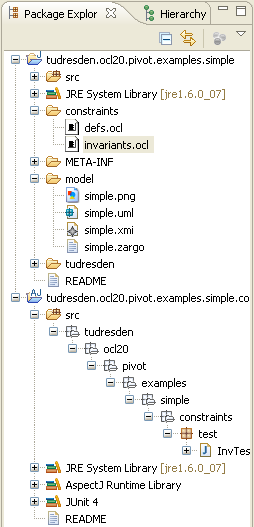
\includegraphics[width=0.5\linewidth]{figures/examples/simple03}
	\caption{The package explorer containing the two projects which are needed to run this tutorial.}
	\label{pic:example:simple03}
\end{figure}

\begin{figure}[!b]
	\centering
	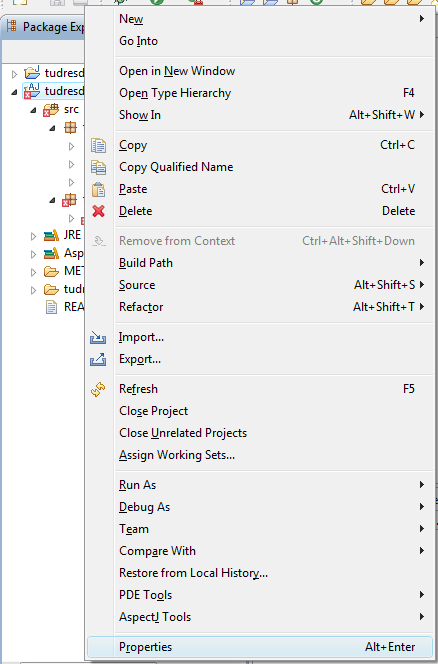
\includegraphics[width=0.8\linewidth]{figures/codegen/properties1}
	\caption{Selecting the properties settings.}
	\label{pic:codegen:properties1}
\end{figure}

After importing the second plug-in, we have to add the JUnit4 library to the project's build path. Right click on the project in the \eclipse{Package Explorer} and select the menu item \eclipse{Properties} (see Figure \ref{pic:codegen:properties1}). In the new opened window select the sub-menu \eclipse{Java Build Path -> Libraries} and click the button \eclipse{Add Library...} (see Figure \ref{pic:codegen:properties2}). In the following window select \eclipse{JUnit}, click \eclipse{Next}, select \eclipse{JUnit 4} and click \eclipse{Finish}. Click \eclipse{OK} to close the project's properties. The project should not contain any compile errors anymore.

\begin{figure}[!htbp]
	\centering
	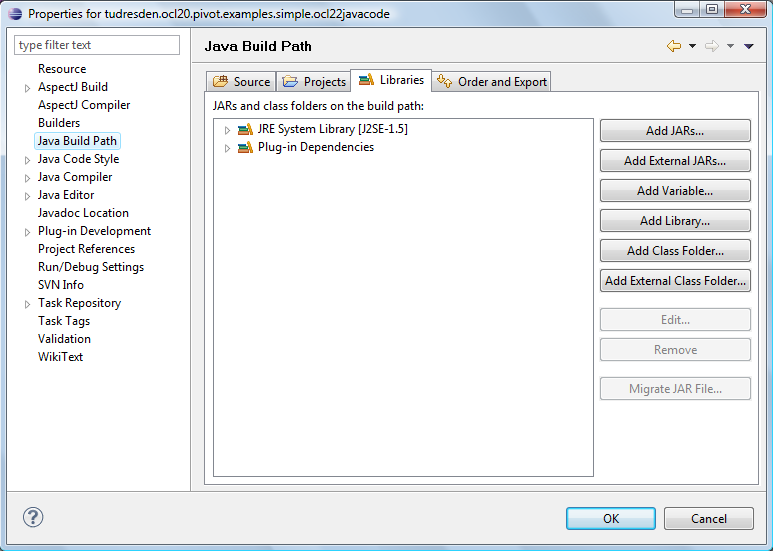
\includegraphics[width=1.0\linewidth]{figures/codegen/properties2}
	\caption{Adding a new library to the build path.}
	\label{pic:codegen:properties2}
\end{figure}

Now we have imported all files we need to run this tutorial. The first project provides a model file which contains the simple class diagram which has been explained in Subsection \ref{intro:simpleExample} (the model file is located at \model{model/simple.uml}) and the constraint file we want to generate code for (the constraint file is located at \model{constraints/invariants.ocl}). Listing \ref{lst:codegen:simpleInvariant} shows one invariant that is contained in the constraint file for which we want to generate code. The invariant declares, that the \model{age} of any \model{Person} must be greater or equal to zero at any time during the life cycle of the \model{Person}.

\lstset{
  language=OCL
}
\begin{lstlisting}[caption={A simple invariant.}, captionpos=b, label=lst:codegen:simpleInvariant, float]
-- The age of Person can not be negative.
context Person
inv: age >= 0
\end{lstlisting}

The second project provides the test class \model{src/tudresden.ocl20.pivot.examples.simple.\linebreak[0]con\-straints.\linebreak[0]InvTest.java} which contains a JUnit test case that checks, whether or not the mentioned constraint is enforced during run-time. The test case creates two \model{Persons} and tries to set their \model{age}. The \model{age} of the second \model{Person} is set to \model{-3} and thus the constraint is violated. The test case expects that a run-time exception is thrown, if the constraint is violated.

The code for the mentioned constraint has not been generated yet and thus the exception will not be thrown. We run the test case by right clicking on the Java class in the \eclipse{Package Explorer} and selecting the menu item \eclipse{Run as -> JUnit Test}. The test case fails because the exception is not thrown (see Figure \ref{pic:codegen:junit01}). To fulfill the test case we have to generate the ApsectJ code for the constraint which enforces the constraint's condition. How to generate such code will be explained in the following.

\begin{figure}[!htbp]
	\centering
	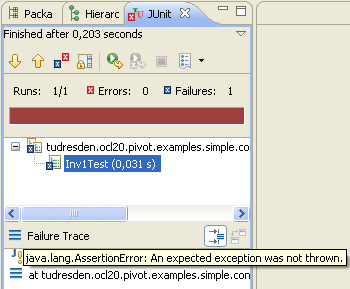
\includegraphics[width=0.6\linewidth]{figures/codegen/junit01}
	\caption{The result of the JUnit test case.}
	\label{pic:codegen:junit01}
\end{figure}



\section{Code Generation}

To prepare the code generation we have to import the model \model{model/simple.uml} into the \eclipse{Model Browser}. We use the import wizard for domain-specific models of the toolkit to import the model. This procedure is explained in the already mentioned introduction in Chapter \ref{chapter:introduction}. Afterwards, we have to import the constraint file \model{constraints/invariant.ocl} which is done by an import wizard again. After the importation, the \eclipse{Model Browser} should look like illustrated in Figure \ref{pic:codegen:modelBrowser}. Now we can start the code generation.

\begin{figure}[!htbp]
	\centering
	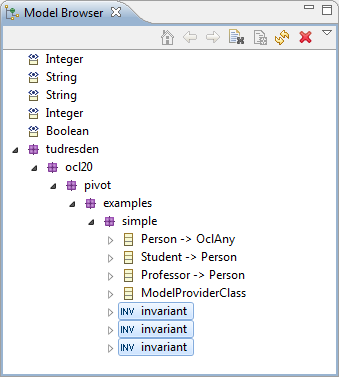
\includegraphics[width=0.6\linewidth]{figures/codegen/modelBrowser}
	\caption{The model browser containing the simple model and its constraints.}
	\label{pic:codegen:modelBrowser}
\end{figure}

To start the code generation we click on the menu item \eclipse{DresdenOCL} and select the item \eclipse{Generate AspectJ Constraint Code}. 


\newpage
\subsection{Selecting a Model}

A wizard opens and we have to select a model for code generation (see Figure \ref{pic:codegen:codegen01}). We select the \model{simple.uml} model and click the \eclipse{Next} button.

\begin{figure}[!b]
	\centering
	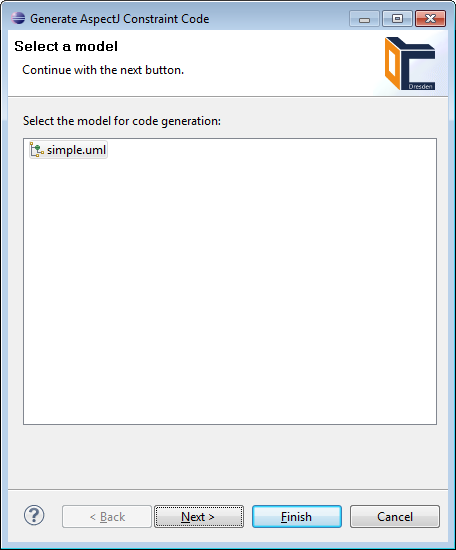
\includegraphics[width=1.0\linewidth]{figures/codegen/codegen01}
	\caption{The first step: Selecting a model for code generation.}
	\label{pic:codegen:codegen01}
\end{figure}


\newpage
\subsection{Selecting Constraints}

As a second step we have to select the constraints for that we want to generate code. We only select the constraint that enforces that the \model{age} of any \model{Person} must be equal to or greater than zero and click the \eclipse{Next} button (see Figure \ref{pic:codegen:codegen02}).

\begin{figure}[!b]
	\centering
	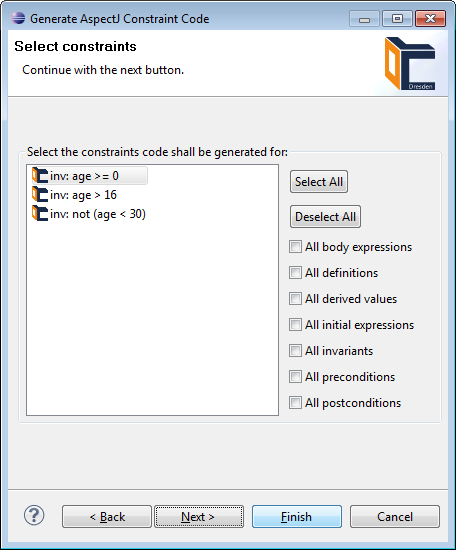
\includegraphics[width=1.0\linewidth]{figures/codegen/codegen02}
	\caption{The second step: Selecting constraints for code generation.}
	\label{pic:codegen:codegen02}
\end{figure}


\newpage
\subsection{Selecting a Target Directory}

Next, we have to select a target directory to that our code shall be generated. We select the source directory of our second project (which is \model{tudresden.\linebreak[0]ocl20.pivot.examples.simple.\linebreak[0]ocl22javacode/src}) (see Figure \ref{pic:codegen:codegen03}). Please note, that we select the source directory and not the package directory into which the code shall be generated! The code generator creates or uses contained package directories depending on the package structure of the selected constraint. Additionally we can specify a sub folder into that the constraint code shall be generated relatively to the package of the constrained class. By default this is a sub directory called \model{constraints}. We don't want to change this setting and click the \eclipse{Next} button.
	
\begin{figure}[!b]
	\centering
	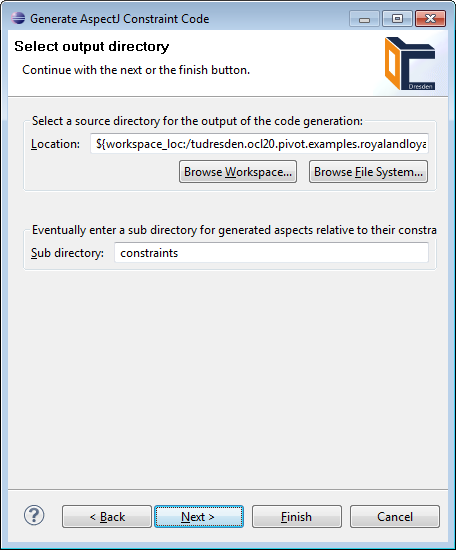
\includegraphics[width=1.0\linewidth]{figures/codegen/codegen03}
	\caption{The third step: Selecting a target directory for the generated code.}
	\label{pic:codegen:codegen03}
\end{figure}


\newpage
\subsection{Specifying General Settings}
	
On the following page of the wizard we can specify general settings for the code generation (see Figure \ref{pic:codegen:codegen04}).

\begin{figure}[!b]
	\centering
	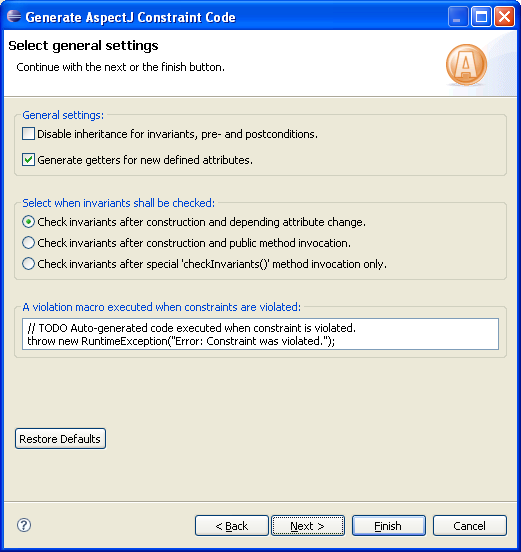
\includegraphics[width=1.0\linewidth]{figures/codegen/codegen04}
	\caption{The fourth step: General settings for the code generation.}
	\label{pic:codegen:codegen04}
\end{figure}

We can disable the inheritance of constraints (which would not be useful in our example because we want to enforce the constraint for \model{Persons}, but for \model{Students} and \model{Professors} as well). We can also enable that the code generator will generate getter methods for newly defined attributes of \model{def} constraints. More interesting is the possibility to select one of three provided strategies, when invariants shall be checked during runtime:

\begin{enumerate}
	\item Invariants can be checked after construction of an object and after any change of an attribute or association which is in scope of the invariant condition (\keyword{Strong Verification}).
	\item Invariants can be checked after construction of an object and before or after the execution of any public method of the constrained class (\keyword{Weak Verification}).
	\item And finally, invariants can only be checked if the user calls a special method at runtime (\keyword{Transactional Verification}).
\end{enumerate}

These three scenarios can be useful for users in different situations. If a user wants to verify strongly, that his constraints are verified after any change of any dependent attribute he should use \keyword{Strong Verification}. If he wants to use attributes to temporary store values and constraints shall only be verified if any external class instance wants to access values of the constrained class, he should use \keyword{Weak Verification}. If the user wants to work with databases or other remote communication and the state of his constraint classes should be only valid before data transmission, he should use the scenario \keyword{Transactional Verification}.

Finally, we can specify a \keyword{Violation Macro} which specifies the code, which will be executed when a constraint is violated during runtime. By default, the violation macro throws a run-time exception. We also want to have a run-time exception thrown when our constraint is violated. Thus, we do not change the violation macro and continue with the \eclipse{Next} button.


\newpage
\subsection{Constraint-Specific Settings}

The last page of the code generation wizard provides the possibility to configure some of the code generation settings constraint-specific by selecting a constraint and adapting it's settings (see Figure \ref{pic:codegen:codegen05}). We don't want to adapt the settings, thus we can finish the wizard and start the code generation by clicking the \eclipse{Finish} button.

\begin{figure}[!b]
	\centering
	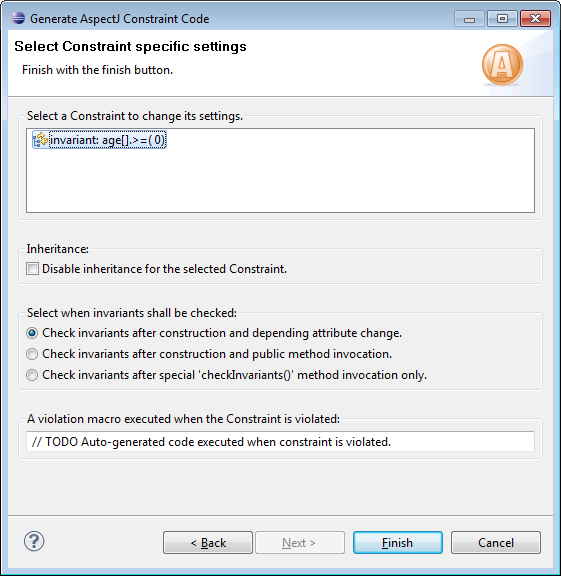
\includegraphics[width=1.0\linewidth]{figures/codegen/codegen05}
	\caption{The fifth step: Constraint-specific settings for the code generation.}
	\label{pic:codegen:codegen05}
\end{figure}



\newpage
\section{The Generated Code}

After finishing the wizard, the code for the selected constraint will be generated. To see the result, we have to refresh our project in the workspace. We select the project \model{tudresden.ocl20.pivot.\linebreak[0]examples.simple.constraint} in the \eclipse{Package Explorer} open the context menu by a right mouse click and select the menu item \eclipse{Refresh}. Afterwards, our project contains a new generated AspectJ file called \model{tudresden.ocl20.pivot.examples.simple.constraints.InvAspect\-01.aj} (see Figure \ref{pic:codegen:packageExplorer}). Now we can rerun our JUnit test case. The test case finishes successfully because the expected run-time exception is thrown (see Figure \ref{pic:codegen:junit02}).	

\begin{figure}[!b]
	\centering
	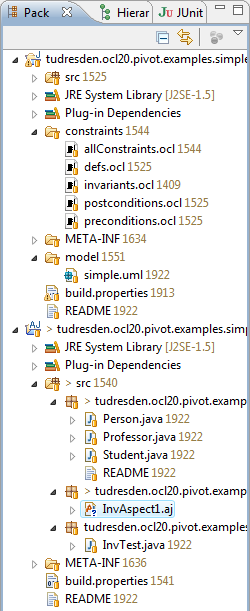
\includegraphics[width=0.5\linewidth]{figures/codegen/packageExplorer}
	\caption{The package explorer containing the new generated aspect file.}
	\label{pic:codegen:packageExplorer}
\end{figure}


\begin{figure}[!htbp]
	\centering
	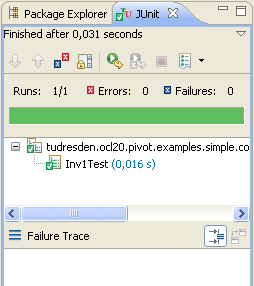
\includegraphics[width=0.5\linewidth]{figures/codegen/junit02}
	\caption{The successfully finished jUnit test case.}
	\label{pic:codegen:junit02}
\end{figure}


	
\section{Summary}
  
This Chapter described how to generate AspectJ code using the \keyword{OCL22Java} code generator of \acl{DOT4Eclipse}. A more detailed documentation of the OCL22Java code generator can be found in the Minor Thesis (Gro�er Beleg) of Claas Wilke \cite{GB:Wilke}.